\documentclass[fleqn,10pt]{wlscirep}
\usepackage{url}
\usepackage{array}
\usepackage{multirow}

\title{Modeling Coevolutionary Dynamics in the \emph{Lobaria pulmonaria} Lichen Symbiosis}

\author[1,2]{Simon Carrignon}
\author[2,3]{Aina Oll\'e-Vila}
\author[4]{Julia N. Adams}
\author[2,3]{Salva Duran-Nebreda}

\affil[1]{Barcelona Supercomputing Center, Carrer de Jordi Girona, 29-31, 08034 Barcelona, Spain.}
\affil[2]{Instituci\'o Catalana per a la Recerca i Estudis Avan\c{c}ats-Complex Systems Lab, Universitat Pompeu Fabra, 08003 Barcelona, Spain.}
\affil[3]{Institut de Biologia Evolutiva (CSIC-Universitat Pompeu Fabra), Passeig Mar\'itim de la Barceloneta 37, 08003 Barcelona, Spain.}
\affil[4]{University of California, Riverside (UCR), Riverside, CA 92521}


\keywords{Lichens, co-evolution,symbiosis}

\begin{abstract}
Lichenization is an evolutionarily and ecologically successful strategy for Ascomycete fungi, resulting in approximately 18,000 lichen species known to date. Although the nature of the lichen symbiosis is still widely debated, many sources agree that the lichen symbiosis represents an ecologically obligate mutualistic interaction whereby the net fitness of all partners is maximized. In order to elucidate the potential factors driving the evolution of the lichen symbiosis and the broader ecological and evolutionary interactions in the \textit{Lobaria pulmonaria} model organism, an agent-based model based on the widely used ECHO framework was constructed. The tag system of ECHO was used to model molecular recognition (receptors and physical embedding) between algae and fungi, two of the partners necessary to reconstitute the \textit{L. pulmonaria} lichen symbiosis. We compared the simulations' results with \emph{L. pulmonaria} microsatellite data and our model reproduced some features of this data. Molecular data have shown that the mode of reproduction significantly affects within-population genetic structure of \textit{L. pulmonaria}, most likely contributing to the modular structure of this population. Our results also show that the interaction type does not significantly alter network metrics (modularity and nestedness), showing that fungal-algal interactions ranging from  parasitic to mutualistic can support a successful or stable biological entity. 


\end{abstract}
\begin{document}

\flushbottom
\maketitle

\thispagestyle{empty}

\section{Introduction}

Lichens are a hyperdiverse symbiotic group of organisms found in nearly every terrestrial ecosystem from the poles to the tropics and grow on diverse substrates, such as rocks (saxicolous) and the bark of trees (corticolous) \cite{nash1996lichen}. The partnership between a fungus (mycobiont) and a photobiont (cyanobacteria, algae, or both) allows the fungus to obtain carbohydrate-rich resources directly from their photosynthetic partner \cite{lutzoni2009lichens}. In turn, the fungus protects the photobiont from desiccation and light intensity, leading to coevolution of the symbionts\cite{hill2009asymmetric} and adaptive radiation into new environments \cite{nash1996lichen}. The obligate symbionts are morphologically and physiologically integrated, resulting in the symbiotic structure known as the lichen thallus \cite{nash1996lichen}. The lichen symbiosis is an evolutionarily and ecologically successful strategy ($>$20\% of fungi are lichenized), resulting in approximately 18,000 lichen species known to date \cite{nash1996lichen,honegger1998lichen}. Although the nature of the lichen symbiosis is still widely debated, many sources agree that the lichen system represents an ecologically obligate mutualistic interaction whereby the net fitness of all partners is maximized~\cite{bronstein1994our,honegger1998lichen}.


The mode of reproduction strongly influences the genetic structure of lichen populations \cite{dal2012vertical}, affecting dispersal and evolutionary rates. The majority of lichens can reproduce asexually and sexually\cite{nash1996lichen}. In the asexual mode of reproduction, mycobionts and photobionts are co-dispersed via fragmentation of the main thallus body or via specialized asexual propagules (isidia or soredia), resulting in genetically identical lichens (vertical  transmission)\cite{nash1996lichen, dal2012vertical}. In the sexual mode of reproduction (horizontal transmission), the fungal spores (i.e. ascospores) are dispersed from specialized sexual structures known as ascomata. The ascospores must find a compatible algae, cyanobacterium, or both in order to reconstitute the lichen thallus (\emph{relichenization}). The compatible photosynthetic partner can either be free-living \cite{sanders2002reproductive} or captured from another lichen \cite{friedl1987thallus}. 


\begin{figure}
\centering
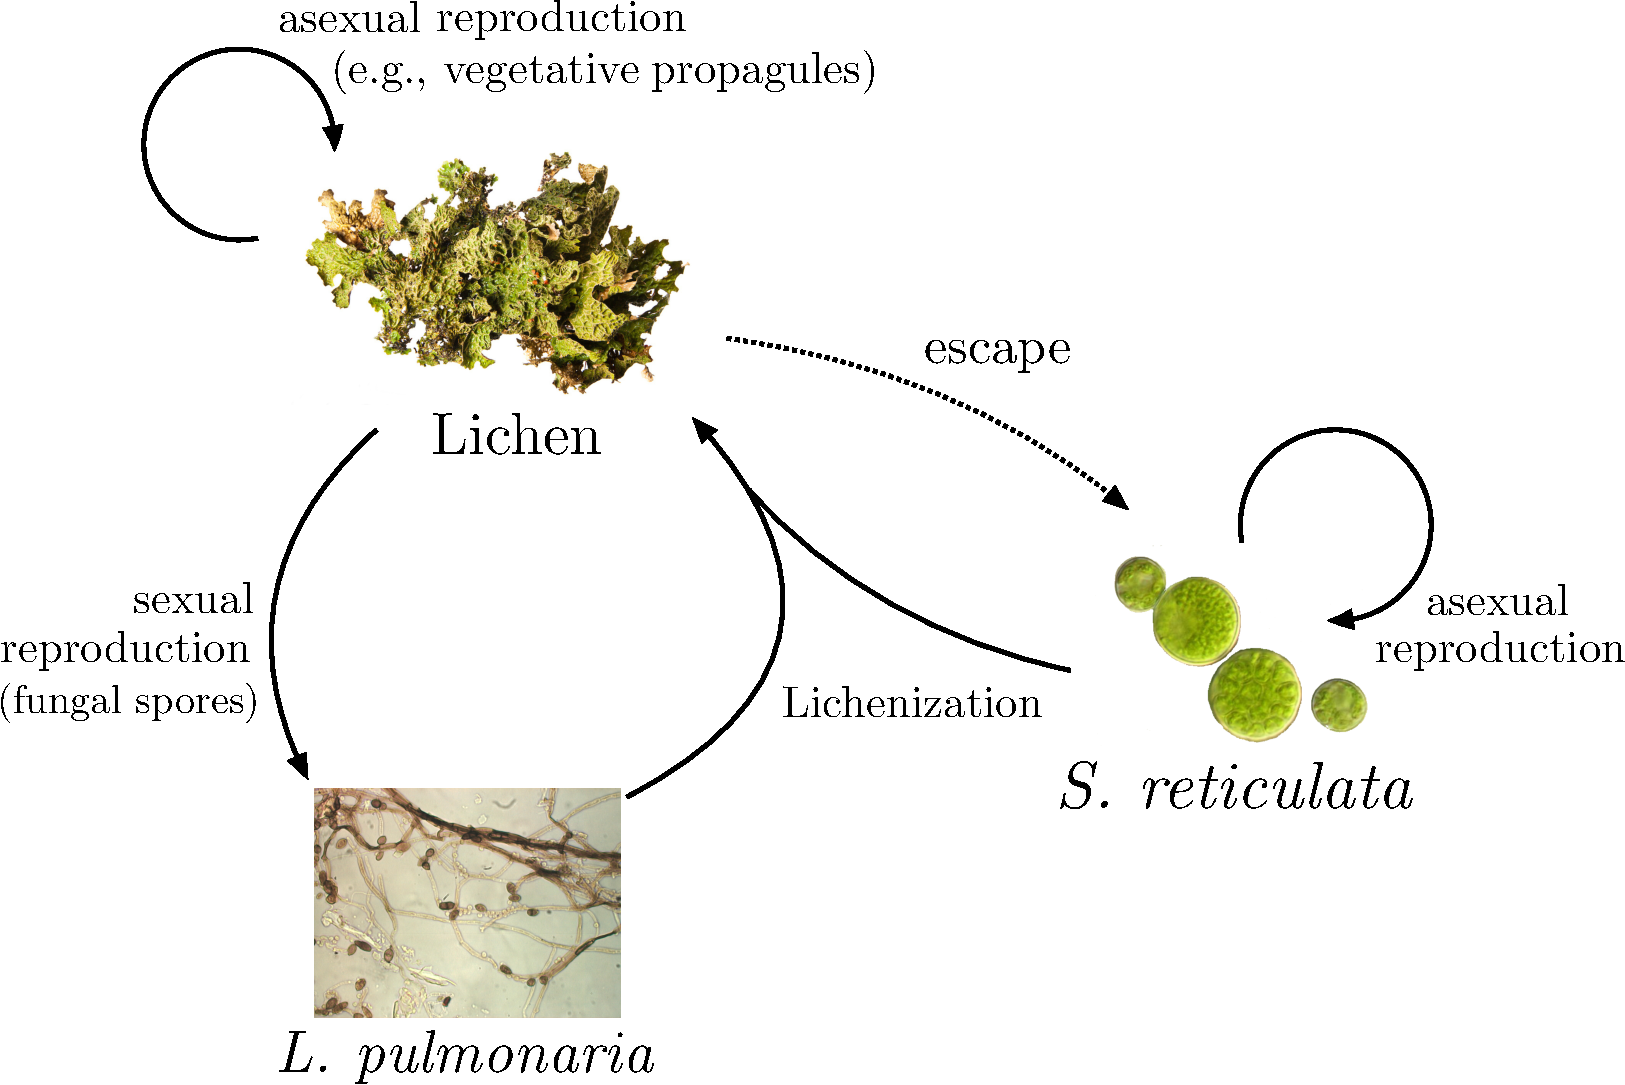
\includegraphics[width=.6\textwidth]{img/interaction_scheme}
\caption{{\bf Life cycle of the {\em L. pulmonaria} system.} Solid arrows represent sexual (via fungal spores) and asexual (e.g., vegetative propagules and thallus fragments) reproductive events, while the dotted arrow represents the process of the algae escaping the partnership via zoospores. Currently, little is known about the free-living status of the photobiont \cite{dal2011phylogeny}. This figure summarizes the known (solid arrows) and inferred (dashed arrows) interactions between the agents of our model. Each process is governed by at least one parameter, some of which have been explored through a sensitivity analysis in our evolutionary algorithm.}
\end{figure}

\textit{Lobaria pulmonaria} is considered the best-studied lichen species worldwide from both an ecological and genetic point of view \cite{grube2012exploring}. The foliose lichen is distributed throughout Europe and parts of North America and grows on the bark of several tree species in old-growth forests \cite{yoshimura1971genus}. \textit{L. pulmonaria} is a lichen with a tripartite system consisting of an association among the green alga \textit{Symbiochloris reticulata} \cite{vskaloud2016taxonomic}, the cyanobacterium \textit{Nostoc sp}., and its main fungal host in Europe, \textit{Lobaria} \cite{dal2011phylogeny} . Recently, it has been shown that the mycobiont of \textit{L. pulmonaria} is mostly dispersed together via vegetative propagules and thallus fragments via asexual reproduction\cite{werth2006effect}, implicating long-term interaction in the symbiosis \cite{walser2001species,werth2006effect,dal2012vertical,werth2012congruent}. In addition, a large majority of fungal and algal pairs were represented by clones \cite{dal2012vertical}. These lines of research have shown evidence of significant within-population genetic structure due to restricted gene flow and vertical photobiont transmission. However, recombination has been shown to occur a small percentage of the time \cite{dal2012vertical}. The sexual mode of reproduction is suspected to play a central role at a larger evolutionary scale. 

Recently, it has been shown that the same green algal photobiont genotype was shared among five co-occurring lichen species in the family of Lobariaceae \cite{dal2011phylogeny}, providing evidence for photobiont exchange. Their results also showed that algal-sharing is ubiquitous throughout the Lobaria community. These results support the photobiont-mediated guild hypothesis, which occurs when photobionts are shared among different lichen species in a community within an evolutionary coherent structure \cite{rikkinen2003ecological}. This mechanistically occurs during the sexual mode of reproduction when fungal spores are dispersed and capture photobionts in other fungal guilds\cite{friedl1987thallus}. This mechanism ensures survival of the photobiont and consequently relichenization of the entire fungal guild \cite{dal2011phylogeny}. This relichenization process could be a successful strategy for genetic recombination, allowing lichens to access wider ecological niches by sharing photobionts among different lichens adapted to diverse local conditions. These loosely integrated functional units, whereby different species can exchange resources and genetics materials, are good candidates to explain the evolutionary success of lichens. They allow different sub-components to evolve more or less independently, at different rates, and under different ecological niches, allowing the whole community to adapt to a wider range of changing environmental conditions.

Empirically studying the evolutionary dynamics of such assemblages is a difficult task because it involves a broad range of heterogeneous entities that co-evolve and interact ecologically at various spatio-temporal scales. Experimental work is also difficult because lichens are fragile biological entities extremely dependent on their local environmental conditions, which are complex and hard to reproduce in the laboratory\cite{nash1996lichen}. One solution to overcome these obstacles is to use computer simulations, which allows the study of a wide range of parameters involving a massive number of heterogeneous entities. The goals of this study were to 1) use microsatellite data \cite{dal2012vertical} of the \textit{L. pulmonaria} lichen system to understand the local processes of dispersion and reproduction of the {\em L. pulmonaria} lichen and 2) model the coevolutionary dynamics between the algal and fungal partners within a lichen under various conditions in a continuous evolutionary algorithm. In order to elucidate the potential factors driving the evolution of the lichen symbiosis and understand broader ecological and evolutionary interactions, this study investigated whether a continuous evolutionary algorithm could reproduce general features of empirical data from 62 populations of \textit{L. pulmonaria} across Europe, America, Asia, and Africa.
\section{Materials and Methods}
\label{sec:mat}
\subsection{Data set}
\label{sec:mat:data}
	We used an available data set from Dal~Grande et al. \cite{dal2012vertical}, which consists of 62 populations of \textit{L. pulmonaria} (1960 thalli in total) in forests throughout Europe, America, Asia and Africa. These populations were genotyped at eight fungal-specific (LPu03, LPu09, LPu15, LPu23, LPu24, LPu25, LPu28) and seven algal-specific microsatellite markers (LPh1-LPh7). This approach allows for the reliable identification of lichen thalli with identical fungal and algal multilocus genotypes and allows for fine-scale marker resolution. This is critical for identifying genetically distinct individuals in populations of the same species \cite{dal2012vertical}. 


\subsection{ECHO model}
\label{sec:mat:echo}

In order to model the coevolutionary dynamics between both partners in a lichen and the process of lichenization we devised some modifications to the ECHO model as defined by John Holland \cite{holland1999echoing} (code in Netlogo available upon request). The ECHO model typically consists of a collection of entities living in a bidimensional spatial domain ($\Omega$), which can move around -typically as random walkers- and interact with one another and with their environment. The interactions among agents can be used to model different kinds of processes -such as mating-, and are driven by locality as well as agent-specific properties, namely the agents' genotypes. The ECHO model is also a continuous genetic algorithm \cite{mitchell1998introduction}; upon reproduction old genotypes are copied with slight mutations, giving rise to quantifiable evolutionary dynamics.  

In this work, we used the tag system of ECHO \cite{holland1999echoing} to model the molecular recognition -receptors and physical embedding- between algae and fungi necessary to create a new lichen. We considered two different lichenization functions based on similarity among the interacting agents' genotypes: sigmoid (hill function with $n=2$) and Michaelis-Menten (saturation dynamics). Additionally, other ecologically relevant features such as dispersal rates were included in the model. Simulations were carried out assuming two types of ecological relations between the algae and fungi: parasitism (only one type of agent benefits from the partnership) and mutualism (both agents benefit).

Finally, the last free parameter explored within the system were the ratios of sexual to asexual reproduction. All possible combinations of ecological interactions and lichenization functions were expanded with varying rates of sexual reproduction ($10^{-2}, 5\times10^{-2},10^{-1},5\times10^{-1},10^0$ times the intrinsic asexual reproduction rates). For each condition in the parameter set, the simulations were run for $10^5$ iterations of the algorithm, and the position in $\Omega$ as well as the genotypes of both the algae and the fungi of every single lichen were recorded. Results reported here stem from a $5$ replicate average.

\subsection{Reconstruction of bipartite networks}
\label{sec:mat:reco}

\begin{figure}
\centering
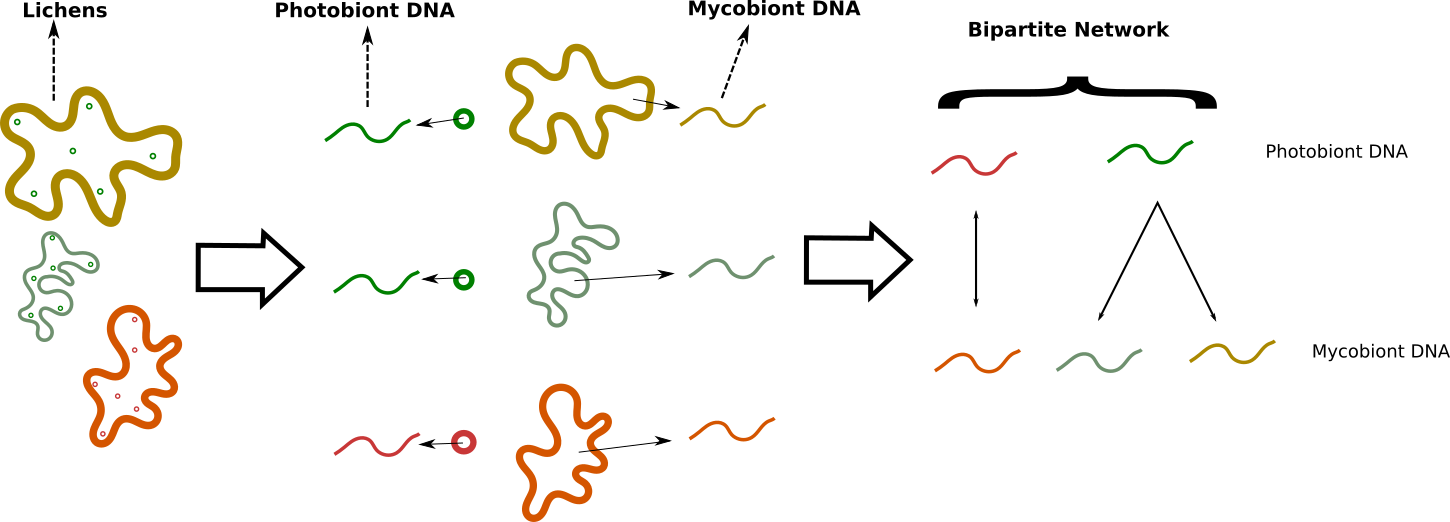
\includegraphics[width=.7\textwidth]{img/bipartite_howto}
\caption{{\bf Construction of a bipartite network of symbionts from sequencing data.} We separated the microsatellite data from the photobiont (algae) and the mycobiont (fungi), and constructed a bipartite network with these two lists. One node corresponds to a unique photobiont multilocus genotypes ($MLG_A$) and the other node corresponds to a unique mycobiont multilocus genotypes ($MLG_F$). Nodes were connected as edges when there was a direct observation of a particular pair ($A_n, F_n$) and when nodes were close in sequence space (see section 2.3).}
\label{fig:bipartite_howto}
\end{figure}

\begin{figure}
\centering
 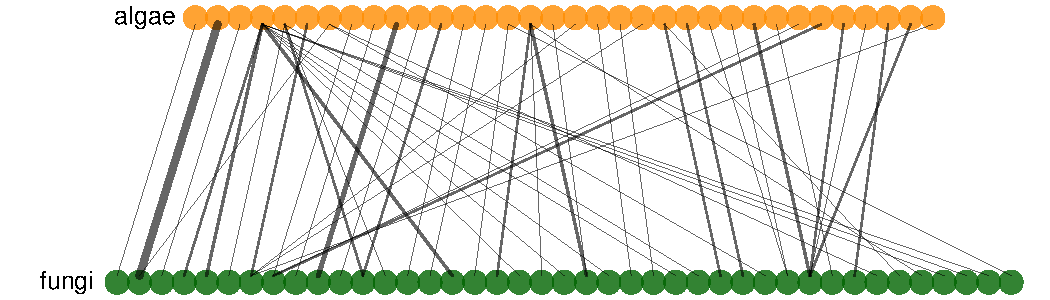
\includegraphics[width=.9\textwidth]{img/bipartite29.pdf}
 
\caption{\textbf{Bipartite network of Algae-Fungi Multilocus Genotypes ($MLG$) interactions from all lichens of the population $\#29$ in the Dal Grande \textbf{}\emph{et al.} dataset\cite{dal2012vertical}}. Each node represents one unique $MLG$, defined by a unique list of microsatellites. Yellow nodes represents the Algae's $MLG$ and green nodes represent the Fungus's $MLG$. A link between two nodes indicates that two MLG's were in symbiosis in at least one lichen. Edge weight (width and the darkness of the link) is directly proportional to the number of times the two $MLG$s have been found in symbiosis together.}
\label{fig:bipartite_ex}

\end{figure}


We separated the lists of algal and fungal microsatellite data \cite{dal2012vertical} to create a bipartite network of the relationships among symbionts. For each algae $A_n$, in symbiosis with a fungus $F_n$, we looked for the existence of another fungus $F_m$ in symbiosis with another algae $A_m$ "similar" to  $A_n$, and created a link between $A_n$ and $F_m$. As a preliminary test, we considered two symbionts as "similar" when they shared the same microsatellites, that is, they represent the same "Multilocus Genotype" ($MLG$). Therefore, we assumed that genetically similar symbionts have a higher probability of sharing the same ancestor. This method, illustrated in Fig.~\ref{fig:bipartite_howto}, allowed us to create a bipartite network of interactions among all the unique $MLG$ of the algae ($MLG_A$) with all the unique $MLG$ of the fungi ($MLG_F$). We generated this graph for each lichen population in the  data set\cite{dal2012vertical} (one example of the resulting network is shown in Fig. \ref{fig:bipartite_ex}) and performed the same analysis with this data set and with the simulations' output (obtained from the model detailed in Section \ref{sec:mat:echo}). In that case, symbionts' \emph{tags} were used to group individuals sharing the same ancestor. 
In the data set by Dal Grande \emph{et al.} \cite{dal2012vertical}, each lichen population contained approximately 32 lichens. At the end of each simulation, the output contained approximately $1\,000$ lichens (depending on the rate of reproduction and other factors). In order to effectively compare the networks extracted from the Dal Grande \emph{et al.} data set\cite{dal2012vertical} and the ones built from the results of our simulations, we performed a scaling on the latter. We normalized the simulations' data set by dividing the output lattice of the model into roughly 60 similar sub-populations (in terms of surface size, \emph{cf.} Fig.~\ref{fig:scaling}). This led to sub-populations with between 5 and 90 lichen samples. We constructed two sets of networks: one where all the lichens from one simulation were considered as a unique population, the other where the simulation output was considered as 60 different populations. Given the population size generated by the simulation described in section~\ref{sec:mat:echo}, we obtained $1\,500$ networks in the first set and $90\,000$ in the second one. In the following sections we use both sets of networks and compared the results retrieved for each data set.

\begin{figure}[ht!]
\centering
\begin{tabular}{m{5cm}|m{3cm} m{1.7cm}}
 Dal Grande et al. 2012 & \multicolumn{2}{l}{Model Output} \\\hline
 
\multirow{3}{*}{ 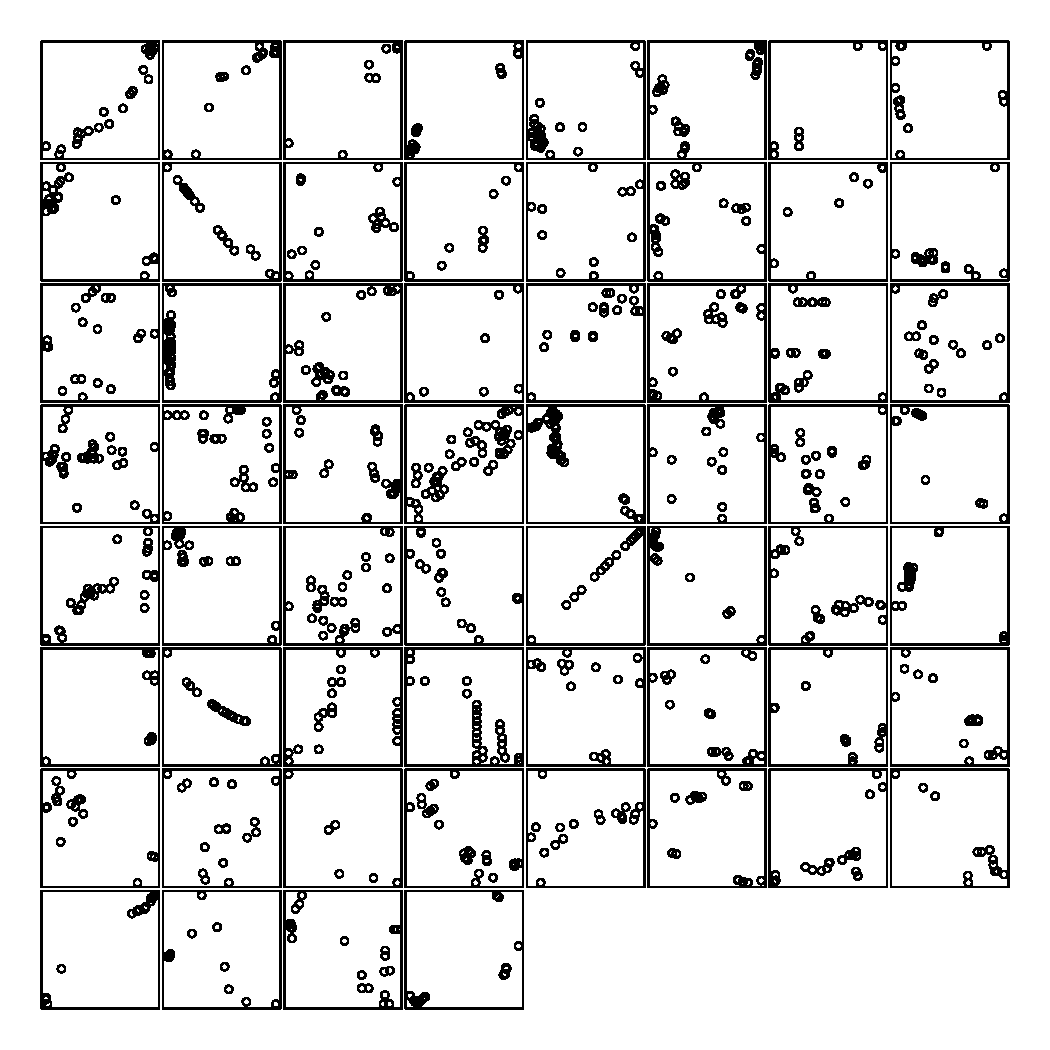
\includegraphics[height=5cm]{img/subsambpl} } &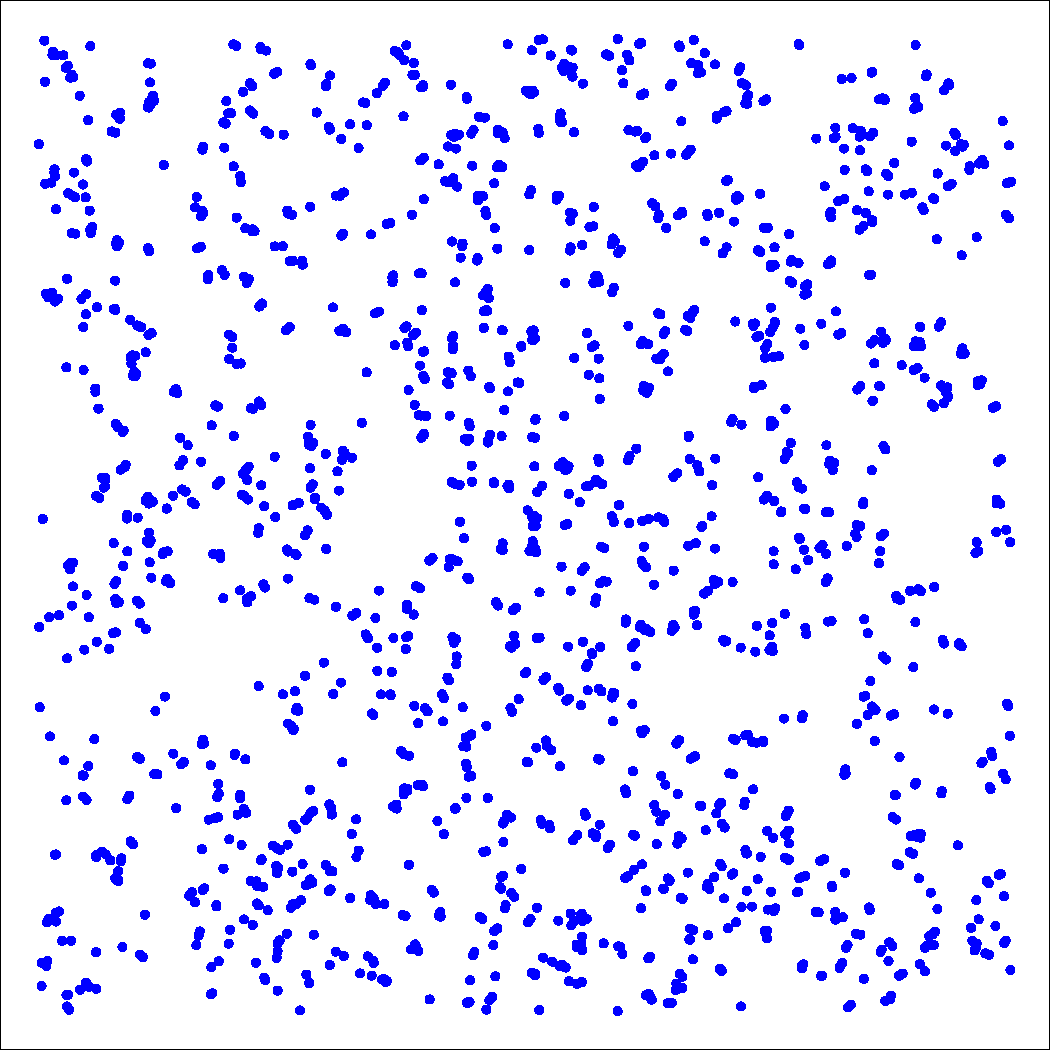
\includegraphics[width=3cm]{img/nosplit}& Non-scaled \\
  &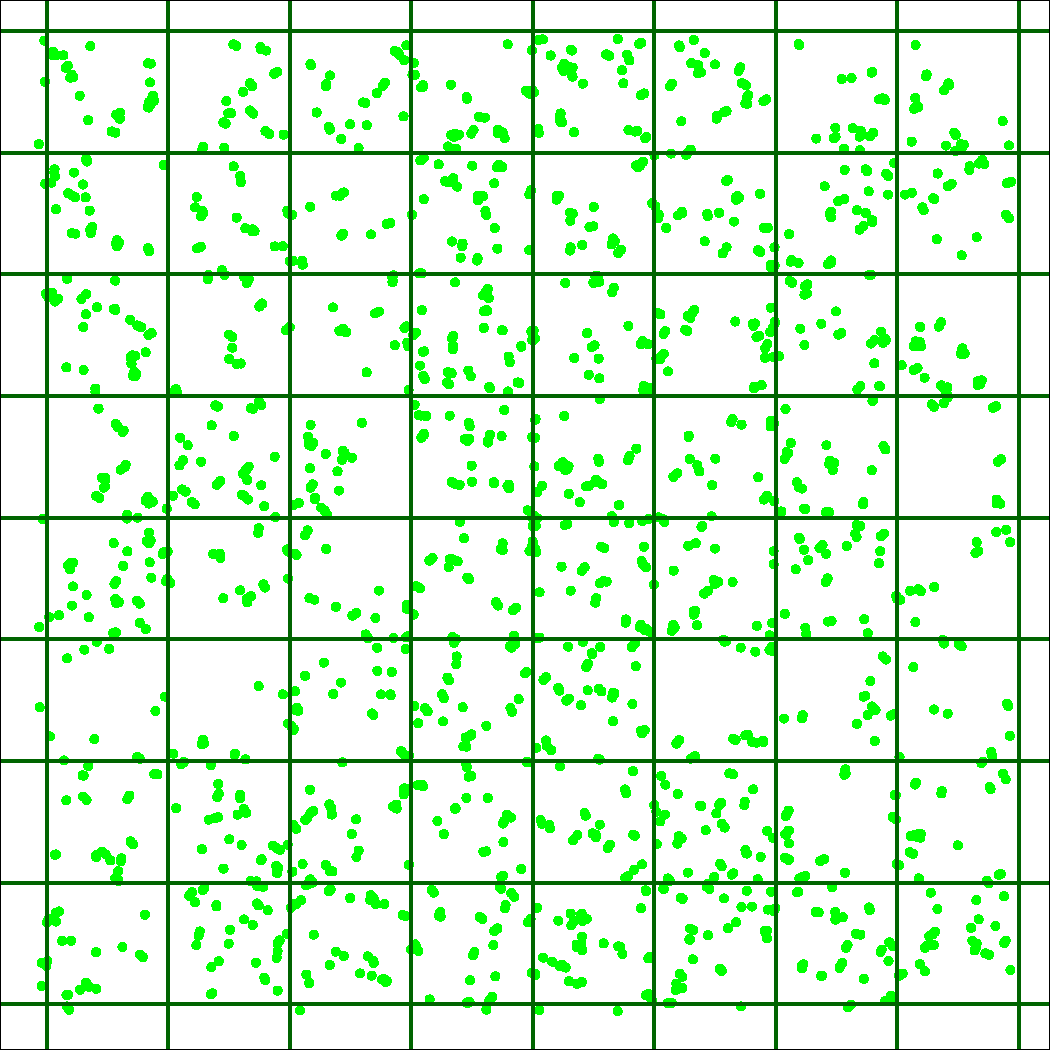
\includegraphics[width=3cm]{img/split}& Scaled  
\end{tabular}
\caption{\textbf{Rescaling of the data in the present study.} The left panel shows the spatial locations of lichen populations from Dal Grande \textit{et al.} 2012 \emph{et al.} \cite{dal2012vertical} side by side. The right panels (non-scaled and scaled) show the spatial locations of lichens after a typical simulation of our model. The bottom right panel shows the artificial separation we added in order to recreate roughly 60 sub-populations. This number is closer to the one found in the original data set.}
\label{fig:scaling}
\end{figure}

\subsection{Network metrics}
\label{sec:mat:net}
\subsubsection{Modularity}
\label{sec:mat:net:mod}
Modularity indicates the presence of dense clusters of nodes with many overlapping interactions embedded within a network. Clusters are considered dense when they have high internal edge density relative to the expected edge density in a null model. 

We used the leading eigenvector method proposed by Newman and Girvan \cite{newman2004finding}, which was later adapted for bipartite networks by Barber \cite{barber2007modularity}. The goal of this method is to maximize the following equation, 

\begin{equation}
Q = \frac{1}{|E|}\sum_{ij} (B_{ij} - \frac{k_id_j}{|E|}\delta(g_i,h_j))
\end{equation}

where ($B_{ij}$ - $\frac{k_id_j}{|E|}$) is the so-called modularity matrix (see Barber 2007\cite{barber2007modularity} for details). With this method, putative modules and the modularity metric within the network were obtained. The software package Bimat \cite{flores2016bimat} was used to compute these metrics.

\subsubsection{Realised Modularity}
Realised modularity is simply defined as the ratio of interactions established between members of the same modules ($L_i$) versus members of different modules ($L_o$)\cite{poisot2013measure} as follows,
\begin{equation}
Q_r = \frac{L_i}{L_o}
\end{equation}
The software package Bimat \cite{flores2016bimat} was also used to compute this metric.

\subsubsection{Nestedness}
\label{sec:mat:net:nest}
Nestedness is a concept borrowed from island biogeography\cite{atmar1993measure}, which describes the extent to which interactions form ordered subsets of each other\cite{bascompte2006structure}. Although there are several proposed metrics for quantifying this property, we used the NODF nestedness metric, which is based on the extent to which a network exhibits decreasing fill and paired overlap. This metric is normalized for matrix size (i.e. takes values between 0 and 1), allowing for comparison of networks of different sizes. A value of 0 indicates the lack of decreasing fill and paired overlap. A value of 1 corresponds to a perfectly nested matrix. The software package BiMAT \cite{flores2016bimat} was used to compute the nestedness of the networks generated from the data set and the model simulations.  The equations  used are shown as follows, 

\begin{equation}
N_{NODF}=\frac{\sum_{ij}M_{ij}^{row}+\sum_{ij}M_{ij}^{col}}{[\frac{m(m-1)}{2}]+[\frac{n(n-1)}{2}]}
\end{equation}
\begin{equation}
M_{ij}^{row} = \begin{cases} 0 & \text{if $k_i \leq k_j$}\\ 
			 n_{ij}/ \text{min$(k_i,k_j)$} & \text{otherwise}\\
\end{cases}
\end{equation}

where $m$ and $n$ are the number of rows and columns, respectively and $k_i$ and $k_j$ are the number of interactions in rows $i$ and$j$. In turn, $n_{ij}$ is the number of shared interactions between rows $i$ and $j$. NODF measures the nestedness of the interaction matrix across rows by assigning a value $M_{ij}^{row}$ to each pair $i,j$ of rows. Positive contributions to NODF require pairs of columns to exhibit decreasing fill, which is satisfied when $k_i>k_j$ -meaning that the degree of node $i$ is bigger than one of node $j$. A similar term $M_{ij}^{col}$ is used to compute column contributions. The total nestedness is the sum of column and row contributions. 


\section{Results}
\label{sec:res}
\subsection{Parasitism versus Mutualism}
\label{sec:res:para}
Parasitic and mutualistic interactions among symbionts show very similar results regarding modularity ($Q_b$), number of modules, realised modularity ($Q_r$) and nestedness (Table~\ref{tab:parasitism-mutualism}). A few values were significantly different, which is most likely due to the high quantity of networks compared. Table~\ref{tab:parasitism-mutualism} shows the mean properties of the networks collected at  $60\,000$ time iterations for the different configurations. Equality between mutualistic and parasitic relationships holds for the entire simulation time (data not shown).


 

% latex table generated in R 3.3.2 by xtable 1.8-2 package
% Thu Jan  5 21:55:33 2017
\begin{table}[ht]
\centering
\begin{tabular}{rcccccccccccc}
  \hline
  & \multicolumn{3}{c}{Number of Module}& \multicolumn{3}{c}{Qr ratio} & \multicolumn{3}{c}{Modularity (Qb)} & \multicolumn{3}{c}{Nestedness} \\
 SRP (\%)& P & M & pval & P & M & pval & P & M & pval & P & M & pval \\\hline
1 & 169.43 & 159.39 & \textbf{0.01} & 0.83 & 0.83 & 0.72 & 0.89 & 0.89 & 0.82 & NA & NA & NA \\
  5 & 75.03 & 74.19 & 0.55 & 0.38 & 0.39 & 0.09 & 0.65 & 0.65 & 0.19 & NA & NA & NA \\
  10 & 53.51 & 54.40 & 0.49 & 0.30 & 0.29 & 0.49 & 0.60 & 0.60 & 0.42 & $<$ 0.01&$<$ 0.01 & 0.83 \\
  50 & 35.77 & 35.76 & 0.99 & 0.25 & 0.24 & 0.02 & 0.57 & 0.56 & \textbf{$<$ 0.01} &$<$ 0.01 &$<$ 0.01 & 0.12 \\
  100 & 34.16 & 34.20 & 0.96 & 0.25 & 0.24 & $\mathbf{<0.001}$ & 0.57 & 0.56 &\textbf{$<$ 0.001}  & $<$ 0.01 &$<$ 0.01 & 0.09 \\
   \hline
\end{tabular}
\caption{\textbf{Comparison of different network properties for simulations with (P) parasitic and (M) mutualistic interactions with different Sexual Rate Percentages (SRP).} Each value represents the mean properties of the networks extracted from the output of the simulation at the $60\,000$th iteration. The same results hold for every iteration of the simulation (data not shown).}
\label{tab:parasitism-mutualism}
\end{table}


\subsection{Impact of sexual reproduction on Fungal-Algal bipartite network modularity}
\label{sec:res:sex}

\subsubsection{Temporal dynamics}
\label{sec:res:sex:temp}
Evolution over time of the modularity and the number of modules in the bipartite networks retrieved from the simulations with different rates of sexual reproduction can be observed in Fig. \ref{fig:dynamic}. We observed how the evolution of modularity and the number of modules across the simulation time varies according to the presence or absence of the grid scaling explained in Section \ref{sec:mat:reco}. Moreover, we observed that the parameter of sexual reproduction percentage (SRP, i.e. the rate of sexual reproduction, \emph{cf.} section~\ref{sec:mat:echo}) plays a role regarding the number of modules and modularity. However, this effect seems to be far more visible at a larger scale.

In the non-scaled grid, regardless of the increase in the number of modules in time, the modularity measure decreases. This decrease can be explained due to a putative regionalization of lichens and algae once the population reaches stability. A co-localization of the species involved in each module could provoke an increase in the number of modules. This could also lead to a decrease in the number of species in each of them. In the scaled-grid, both the number of modules and modularity increases. The putative reason could be that initially we detect very few modules inside the grid spots. Modules would be detected when species within a module start to co-localize, causing an increase either in the number of modules and modularity measures. This could explain the \emph{a priori} contradiction observed in the non-scaled grid.

The same figure shows the influence of sexual reproduction percentage in the temporal dynamics of these measures. The increase or decrease in the percentage of sexual reproduction does not seem to deeply affect the evolution of the number of modules or modularity at a local scale; however, this is not the case of the population at a large scale. In the latter case, a small increase in the rate of sexual reproduction is enough to drastically reduce the number of modules observed in the bipartite network as well as their modularity. The number of modules is roughly divided by $3$ when increasing the rate of sexual reproduction from $1\%$ to $5\%$ (from a mean of around $150$ modules per network to a mean of around $60$ modules), while the modularity decrease from $90\%$ to $65\%$ with the same increase.

The statistical significance of the differences observed in the temporal plots when simulations reach equilibrium can be seen in Figure~\ref{fig:modules}.

\begin{figure}[ht!]
\centering
\begin{tabular}{cc}
   Non-Scaled &  Scaled \\
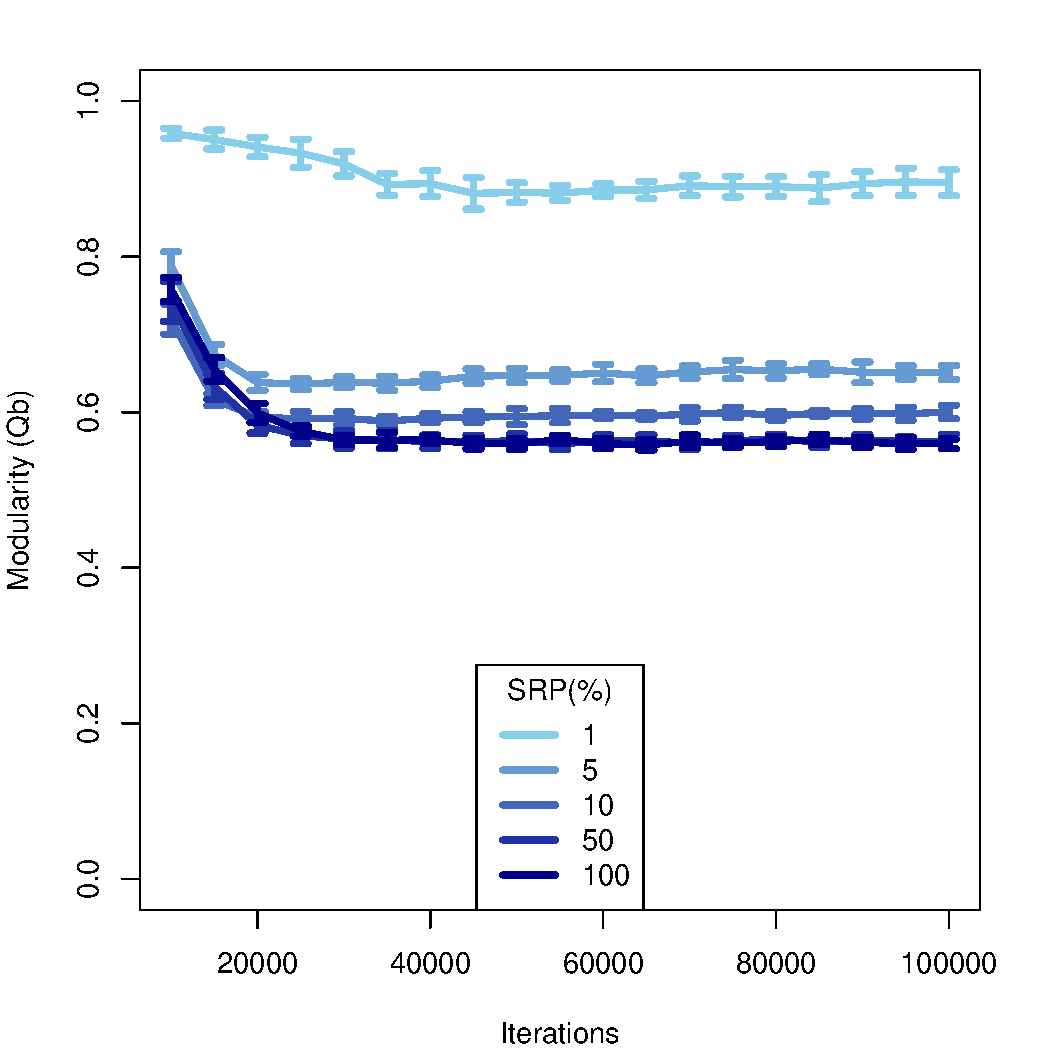
\includegraphics[width=.4\linewidth]{img/QbMetOverTimeFULL.pdf} &
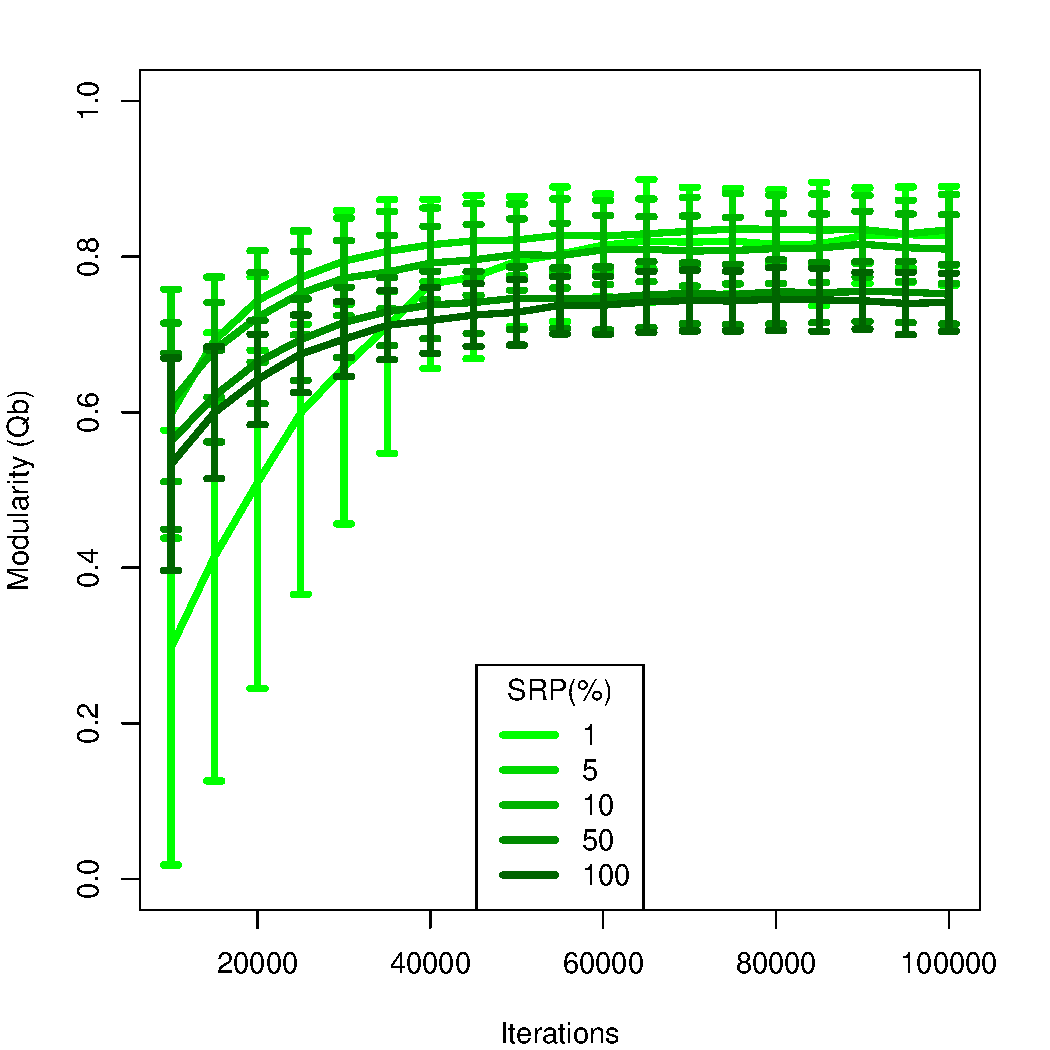
\includegraphics[width=.4\linewidth]{img/QbMetOverTimeRESC.pdf} \\
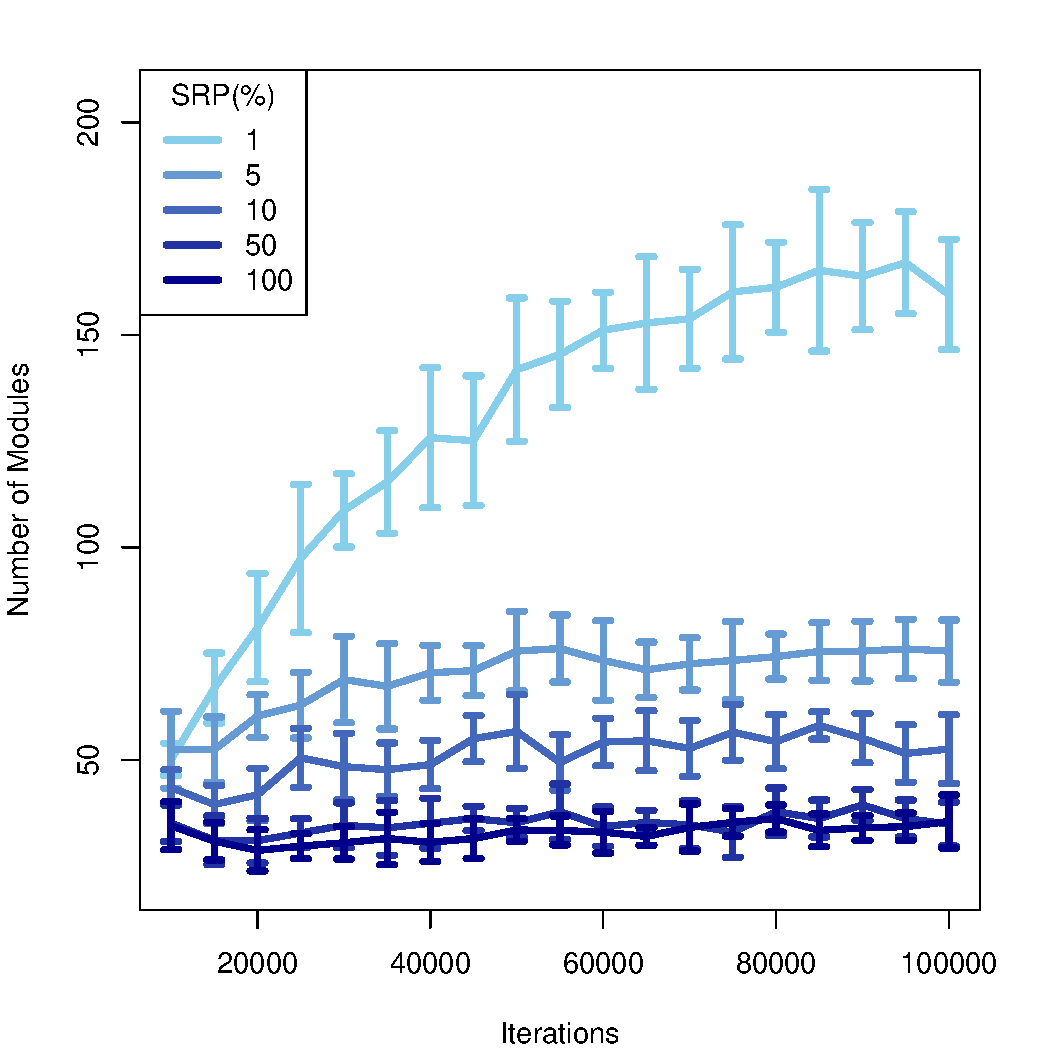
\includegraphics[width=.4\linewidth]{img/NumModuleOverTimeFULL.pdf}	&
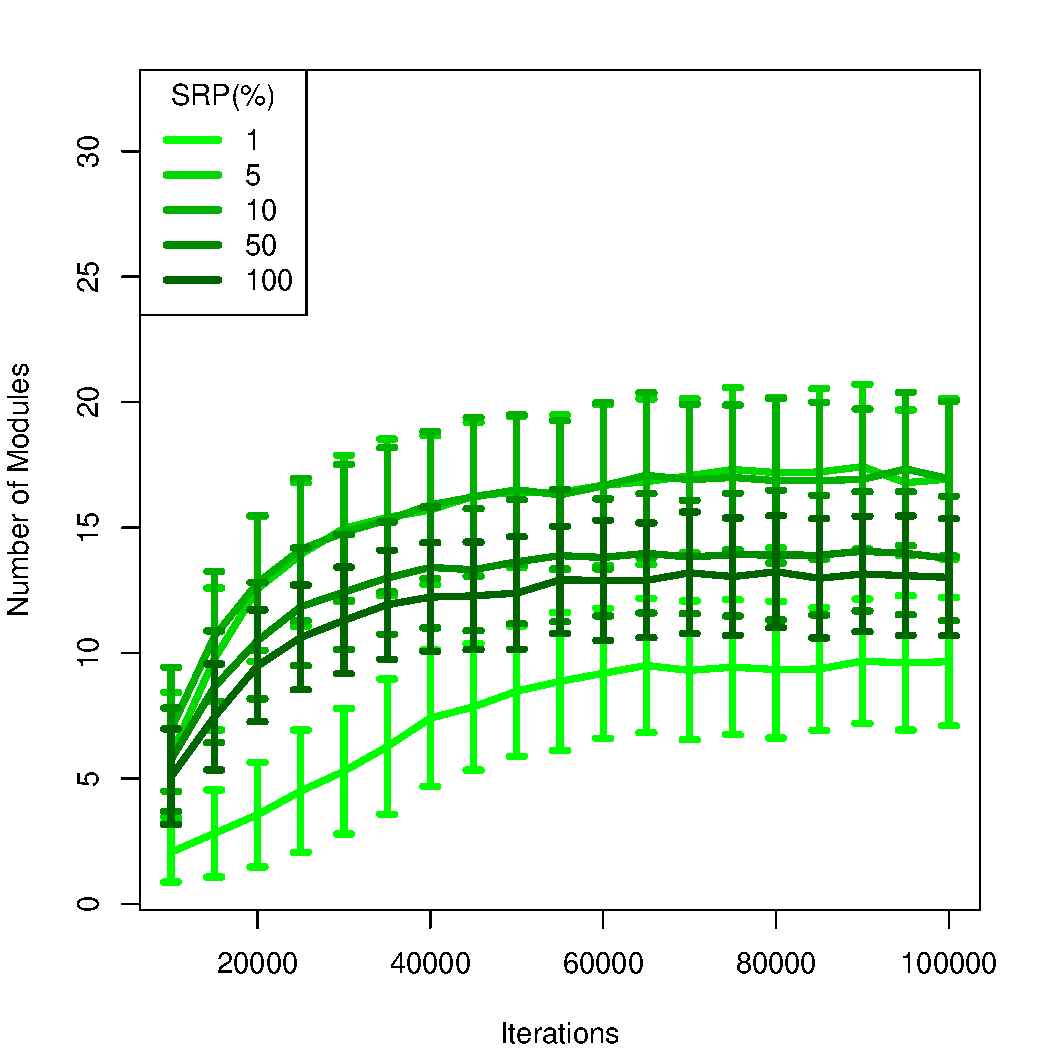
\includegraphics[width=.4\linewidth]{img/NumModuleOverTimeRESC.pdf}\\
\end{tabular}
\caption{\textbf{Evolution over time of the modularity (top) and of the number of modules (bottom) in the bipartite networks found in simulations with different rates of Sexual Reproduction Percentage (SRP).} The blue curves (left) correspond to the properties of networks that build upon the whole simulation, while the green curves (right) correspond to the properties of networks that build upon scaled sub-population.}
\label{fig:dynamic}
\end{figure}



\subsubsection{Comparison with real data}


\label{sec:res:sex:comp}
\begin{figure}[ht!]
\centering
\begin{tabular}{cc}
   Modularity & Number of Module \\
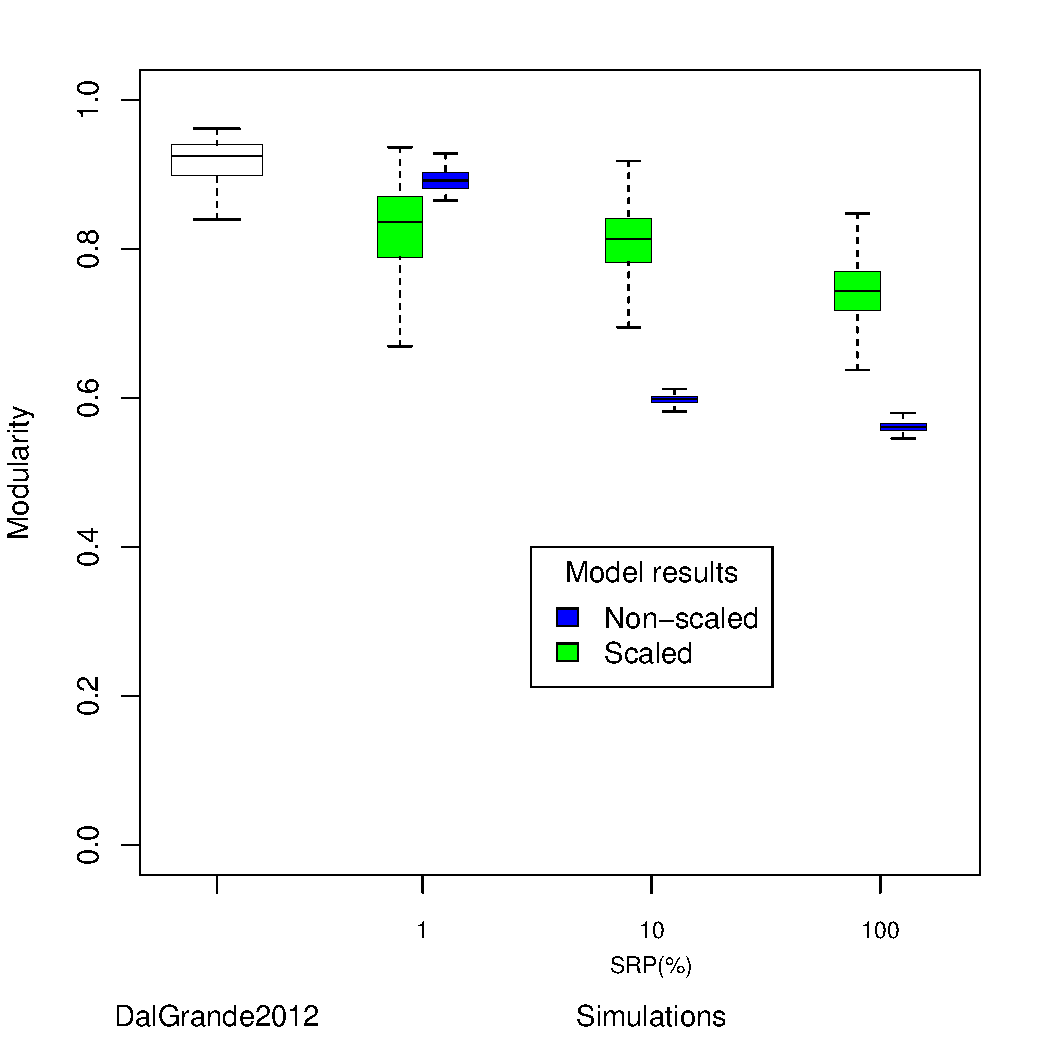
\includegraphics[width=.4\linewidth]{img/QbMetcompare.pdf} &
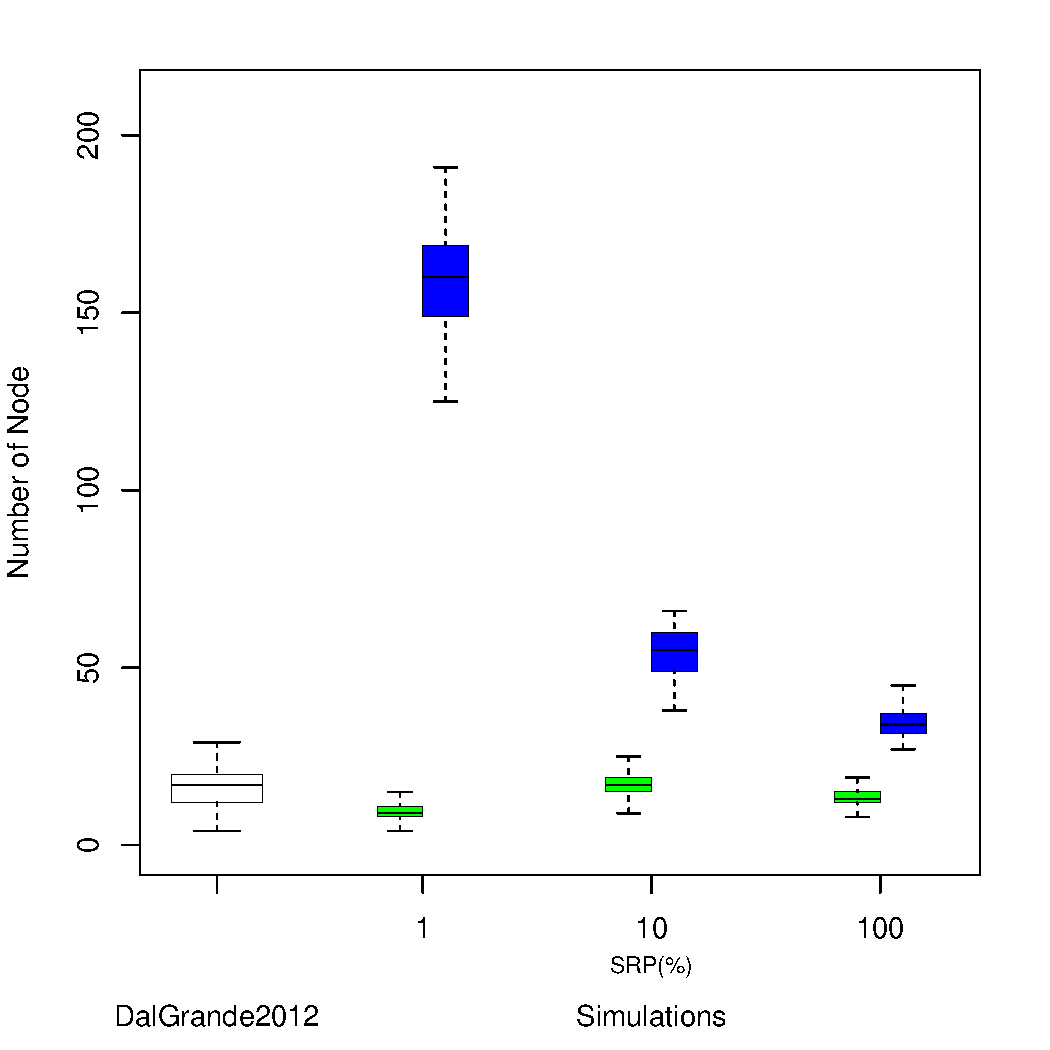
\includegraphics[width=.4\linewidth]{img/NestedNODFcompare.pdf}\\
\end{tabular}
\caption{\textbf{Comparison of the modularity (left) and of the number of modules (right) in the bipartite networks observed in the data set of Dal Grande \emph{et al.}\cite{dal2012vertical} with the networks at the end of the simulations for increasing sexual reproduction rate.} The blue bloxes correspond to the properties of the networks that build upon the whole simulation (non-scaled), the green boxes correspond to the properties of networks that build upon scaled sub-population.}
\label{fig:modules}
\end{figure}

In order to validate our model, we compared the number of modules and the modularity metric observed in the simulations with real data. In Fig.~\ref{fig:dynamic}, we observed that in almost all cases the simulations reach equilibrium after around $60\,000$ iterations. Therefore, we compared the values in Fig. \ref{fig:modules} of those network metrics after $60\,000$ iterations to the ones in the network built from the Dal Grande \emph{et al.} data set. As was done for the temporal analysis, we compared both sets of networks (see section~\ref{sec:mat:net}) resulting from the simulation with networks built from the entire population (non-scaled, in blue) and the networks built from sub-populations (scaled, in green).


For both metrics (modularity and number of modules) results are closer to the real data when the networks are scaled. This should be expected, as the rescaled populations are comparable in size to the populations in the original data set. For the rescaled set of networks, the sexual rate of reproduction does not have a major impact. Nonetheless, the lower SRP rate ($1_\%$) matches more closely to the results from the real data. Interestingly, the major impact regarding the sexual reproduction rates occurs in the non-scaled population. Overall, the networks obtained from the scaled model appear to succesfully reproduce the modular structure of the dataset.

\section{Discussion}
  In this work, we proposed an ECHO-like model encompassing the basic interactions between fungi and algae in order to better understand the evolutionary dynamics of lichenization. Specifically, we explored several parameters of the model that are typically regarded as influential in coevolutionary systems in general and {\em L. pulmonaria} in particular, such as the type of ecological interaction ({\em i.e.} parasitism or mutualism) and the presence of sexual reproduction used conjointly with propagule formation or other modes of asexual reproduction. 

As previously stated, the nature of the ecological interaction between the two partners appears to have little relevance in deciding the general features of the reconstructed genotype-genotype bipartite network, both in terms of nestedness and modularity measures. These results stand in stark contrast to a body of literature that traditionally equates mutualistic bipartite networks to nested structures \cite{bascompte2006structure}, typically through an increased biodiversity \cite{bascompte2006asymmetric} and stability \cite{rohr2014structural} of the ecosystem. 

On the other hand, as initially explored by Dal Grande {\em et al.} \cite{dal2012vertical}, sexual reproduction does appear to have an impact on the population structure of lichens. In particular, we observed that it can drastically change the dynamics as well as the endpoint values of some network metrics under small changes in the incidences of sexual reproduction. Consistent with previous studies \cite{dal2012vertical} using spatial and genetic information, we have found that lower values (in-model value of $10^{-2}\times$ asexual reproduction rates) are the most consistent with the experimental data.

 
The rationale behind such low sexual reproduction rates are still poorly understood. A common hypothesis argues that sexual reproduction could be central to the persistence and evolution of the so-called "photobiont-mediated guilds" \cite{rikkinen2003ecological, dal2011phylogeny}. Our study at two different scales suggests that, although the role of sexual reproduction does not have a huge impact on the interaction properties at the local level (Fig. ~\ref{fig:dynamic}, left), it does have an impact on the temporal dynamics of the bipartite system at a large scale (Fig. ~\ref{fig:dynamic}, right). Our results are consistent with the photobiont-mediated guilds hypothesis, whereby sexual reproduction via algal-sharing among fungal guilds has an important role at a larger evolutionary scale. 
 
 
Switching smoothly from a local to a global scale on real networks is a difficult task, as it is often hard to know how to sample both scales meaningfully. Given the fact that our model can successfully reproduce well-known local properties \emph{cf.} Fig. ~\ref{fig:modules}, we think it also is a good candidate to study the photobiont-mediated guilds -complex entities where different species co-evolve symbiotically and asymbiotically at different tempos and scales.

In reality, a lichen organism faces multiple evolutionary pressures due to environmental conditions from local environmental conditions (e.g., temperature, precipitation, and altitude), stochastic and deterministic environmental factors, and biotic interactions. Therefore, this model can be expanded in several meaningful ways. First, we confined ourselves to model an essentially static two species system. However, in order to study multi-species systems such as photobiont-mediated guilds, the model should be scaled up to larger spatial areas. In doing so, lichen properties such as reproduction and mutation rates, and types of ecological interactions can evolve, leading to the emergence of speciation events. In addition, scaling the model to larger spatial areas is important to understand the role that biogeography plays in the diversification of mycobionts and photobionts. For the sake of simplicity, we did not introduce any anisotropy (humidity or available sunlight for instance) or terrain complexity \cite{atmar1993measure}. However, in an attempt to understand networks involving species interacting at different spatial scales, diversity of local environmental conditions should be included, as it is expected to play an important role in the evolutionary ecology of lichen communities. The model also does not include biotic interactions such as predation by arthropods and vertebrates and competition for space and resources by lichens, bryophytes and fungi. In the future, spatio-temporal variability of species interactions should also be included, as it is also expected to play an important role in the evolutionary dynamics of lichen populations.  


Thus far, our work has shown to successfully model simple dynamics at different scales of a lichen system, in which the coevolutionary dynamics are still poorly understood. Therefore, we not only expect this work to strengthen the current knowledge of the coevolutionary dynamics of the \emph{Lobaria Pulmonaria} system, but also to give insight into a more general understanding of coevolutionary systems whereby a set of species interact and form loosely defined emergent levels of biological organization. 


\section*{Acknowledgements}
This work was initiated at the 2016 Complex Systems Summer School (CSSS) at the Sante Fe Institute (SFI). The authors would like to thank all SFI resident faculty members, SFI external faculty members, SFI Omidyar Postdoctoral Fellows, and 2016 CSSS course participants for productive discussions as well as SFI staff during the 2016 CSSS. The authors would also like to thank Dr. Christoph Scheidegger for access to multiple data sets and Dr. Francesco Dal Grande for providing detailed knowledge of the \emph{L. pulmonaria} system. 

\bibliography{biblio}

\end{document}
